\section{Экспериментальная установка}

\begin{wrapfigure}[18]{r}{0.4\textwidth}
	\centering
	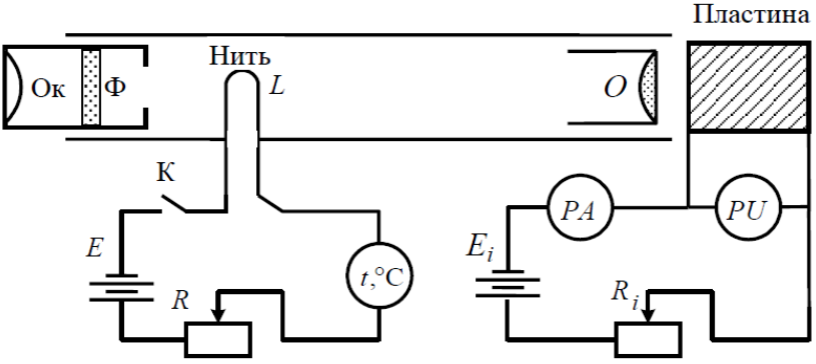
\includegraphics[width=0.38\textwidth]{ExperimentalSetup.png}
	\caption{Схема установки}
	\label{fig:setup}
\end{wrapfigure}

Экспериментальная установка (рис. \ref{fig:setup}) состоит из источника света 1 (ртутная лампа), гониометра 4 и дифракционной решетки 6. Излучение лампы освещает щель 2 коллиматора 3 гониометра и дифракционную решетку, установленную в держателе 5 перпендикулярно падающим лучам. Зрительная труба 9 гониометра может поворачиваться вокруг вертикальной оси гониометра. В фокальной плоскости окуляра зрительной трубы наблюдается дифракционный спектр. Угловое положение зрительной трубы определяется по шкале 7 и нониусу 8 лимба гониометра. Цена деления шкалы гониометра 30', нониуса – 1'. Поскольку начало отсчета по шкале гонио метра может не совпадать с направлением нормали к поверхности решетки, то угол дифракции $\varphi_m$ определяется разностью двух угловm $\alpha_m - \alpha_0$ , где $\alpha_0$ – угол, отвечающий центральному $m = 0$ дифракционному максимуму.

